\documentclass[__main__.tex]{subfiles}

\begin{document}

\qtitle{С}{08}
Примените теорему Гаусса к расчету электростатических полей: найдите поле, порождаемое бесконечной равномерно заряженной (поверхностная плотность заряда $\sigma$) плоскостью, бесконечной равномерно заряженной нитью (линейная плотность заряда $\kappa$).\\

\textbf{Поле, порожденное бесконечно равномерно заряженной плоскостью}\\
 Поверхностная плотность заряда на произвольной плоскости площадью S определяется по формуле:\\
 \begin{gather}
 \sigma = \frac{dq}{dS}
 \end{gather}
 где $dq$ - заряд, сосредоточенный на площади $dS$; $dS$ - физически бм участок поверхности.\\
 Пусть $\sigma$ во всех точках плоскости $S$ одинакова. Заряд $q$ – положительный. Напряженность во всех точках будет иметь направление, перпендикулярное плоскости $S$.\\
 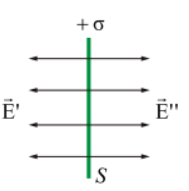
\includegraphics[scale = 1]{C08-1}\\
 Очевидно, что в симметричных, относительно плоскости точках, напряженность $\vec{E}$ будет одинакова по величине и противоположна по направлению. \\
 Представим себе цилиндр с образующими, перпендикулярными плоскости, и основаниями $\triangle S$, расположенными симметрично относительно плоскости.\\
 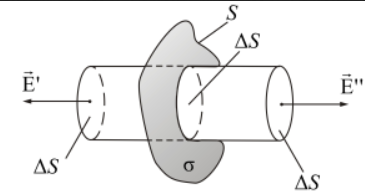
\includegraphics[scale = 1]{C08-3}\\
 Тогда $E' = E'' = E$.\\
 Применим теорему Гаусса. Поток $\Phi_E$ через боковую часть поверхности цилиндра равен нулю, т.к. $E_n = 0$. Для основания цилиндра $E_n = E$.\\ 
 Суммарный поток через замкнутую поверхность (цилиндр) будет равен:\\
 \begin{gather}
 \Phi_E = 2\triangle SE
 \end{gather}
 Внутри поверхности заключен заряд $q = \sigma \triangle S$. Следовательно, из теоремы Гаусса получим: 
 \begin{gather}
 \Phi_E = \frac{q}{\epsilon_0} = 2\triangle SE = \sigma \triangle S \frac{1}{\epsilon_0}
 \end{gather}
 откуда видно, что напряженность поля плоскости $S$ равна: 
 \begin{gather}
 E = \frac{\sigma}{2\epsilon_0}
 \end{gather}
 Полученный результат не зависит от длины цилиндра. Это значит, что на любом расстоянии от плоскости $E = const$.\\
 \textbf{Поле, порожденное бесконечно равномерно заряженной нитью}\\
 Пусть поле создается бесконечной цилиндрической поверхностью радиуса $R$, заряженной с постоянной линейной плотностью $\kappa = \frac{dq}{dl}$, где $dq$ – заряд, сосредоточенный на отрезке цилиндра.\\
 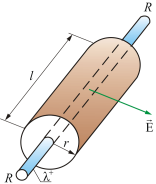
\includegraphics[scale = 0.8]{С08-2}\\
 Из соображения симметрии следует, что $E$ в любой точке будет направлена вдоль радиуса, перпендикулярно оси цилиндра.\\
 Представим вокруг цилиндра (нити) коаксиальную замкнутую поверхность (цилиндр в цилиндре) радиуса $r$ и длиной $l$ (основания цилиндров перпендикулярно оси). Для оснований цилиндров $E_n = 0$  для боковой поверхности $E_n = E(r)$ т.е. зависит от расстояния $r$.\\ 
 Следовательно, поток вектора $\vec{E}$ через рассматриваемую поверхность, равен $\Phi_E = E(r)S = E(r)2\pi rl$.\\
 При $r \leq R$  на поверхности будет заряд $q = \kappa l$. По теореме Гаусса $E(r)2\pi rl = \frac{\kappa l}{\epsilon_0}$, отсюда:\\
 \begin{gather}
 E(r) = \frac{\kappa}{2 \pi \epsilon_0 r}, \qquad \text{при} r\leq R
 \end{gather} 
 Если  $r<R$, $E(r) = 0$ , т.к. внутри замкнутой поверхности зарядов нет.\\
 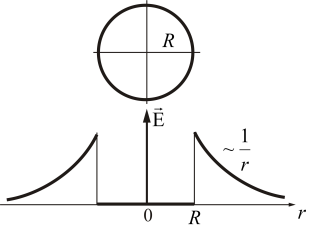
\includegraphics[scale = 4]{С08-4}\\
 Если уменьшать радиус цилиндра R (при $\kappa = const$), то можно вблизи поверхности получить поле с очень большой напряженностью и, при $R \to 0$, получить нить. \\
\end{document}